\chapter{Cơ sở lý thuyết và các công trình liên quan}
\label{chap:related}

Chương này trình bày nền tảng lý thuyết và các công trình liên quan làm cơ sở cho
phương pháp được đề xuất. Trước hết, chúng tôi khảo sát kiến trúc Transformer cùng dòng
mô hình Encoder-only đã trở thành chuẩn mực cho các bài toán hiểu ngôn ngữ
(Mục~\ref{sec:transformer}). Tiếp theo, chúng tôi trình bày các đặc điểm chính của NeoBERT
-- mô hình nền mà đề tài kế thừa -- cùng những cải tiến có ảnh hưởng trực tiếp tới hướng
chuyển giao tiếng Việt (Mục~\ref{sec:neobert}). Sau đó, chúng tôi trình bày cơ sở hình học
của không gian biểu diễn, bài toán thích nghi ngôn ngữ và các phương pháp khởi tạo nhúng
xuyên ngôn ngữ, dẫn tới kỹ thuật Semantic Aware Linear Transfer (SALT) mà đề tài áp dụng
(Mục~\ref{sec:transfer}). Cuối cùng, chương đưa ra một số nhận xét định hướng cho phương pháp
được trình bày ở chương tiếp theo.

% ======================================================================
\section{Kiến trúc Transformer và mô hình Encoder-only}
\label{sec:transformer}

\subsection{Cơ chế tự chú ý trong kiến trúc Transformer}
\label{subsec:attention}

Transformer được Vaswani và cộng sự~\cite{vaswani2017attention} giới thiệu như một kiến
trúc xử lý chuỗi không dùng hồi tiếp. Thay vì đọc token tuần tự như RNN/LSTM, Transformer
cho phép mỗi vị trí quan sát trực tiếp các vị trí còn lại thông qua cơ chế tự chú ý
(self-attention). Đây là lý do kiến trúc này vừa song song hóa tốt trên GPU, vừa học được
các phụ thuộc xa trong câu.

Với ma trận trạng thái ẩn $X$, mô hình tạo ba phép chiếu tuyến tính gồm truy vấn $Q$, khóa
$K$ và giá trị $V$. Trọng số chú ý được tính bằng tích vô hướng có tỷ lệ:
\begin{equation}
  \label{eq:attention}
  \mathrm{Attention}(Q, K, V) = \mathrm{softmax}\!\left(\frac{QK^\top}{\sqrt{d_k}}\right) V
\end{equation}
Trong đó, ma trận $QK^\top$ biểu diễn mức liên hệ giữa mọi cặp token. Vì ma trận này có
kích thước $n \times n$, chi phí chú ý tăng theo $O(n^2)$ khi độ dài chuỗi tăng. Đây là một
lý do các Encoder hiện đại cần kết hợp thêm kỹ thuật tối ưu bộ nhớ như FlashAttention khi
mở rộng ngữ cảnh lên hàng nghìn token.

Transformer thường dùng tự chú ý đa đầu (Multi-Head Attention) để học nhiều kiểu quan hệ
song song. Công thức tổng quát được viết gọn như sau:
\begin{equation}
  \label{eq:mha}
  \begin{aligned}
    \mathrm{MultiHead}(Q,K,V)
      &= \mathrm{Concat}(\mathrm{head}_1,\ldots,\mathrm{head}_h)\,W^O, \\
    \mathrm{head}_i
      &= \mathrm{Attention}(QW_i^Q,\,KW_i^K,\,VW_i^V).
  \end{aligned}
\end{equation}
Sau attention, mỗi khối Transformer còn có mạng truyền thẳng theo vị trí, kết nối tắt và
lớp chuẩn hóa. Các biến thể hiện đại chủ yếu khác nhau ở cách mã hóa vị trí, loại chuẩn hóa
và hàm kích hoạt. Những điểm này sẽ được dùng để giải thích NeoBERT ở Mục~\ref{sec:neobert}.

\subsection{BERT và mô hình hóa ngôn ngữ có mặt nạ}
\label{subsec:bert}

Từ phần encoder của Transformer, Devlin và cộng sự~\cite{devlin2019bert} đề xuất BERT
(Bidirectional Encoder Representations from Transformers). BERT là mô hình Encoder-only:
nó không có bộ giải mã tự hồi quy và không dùng mặt nạ nhân quả, nên mỗi token có thể khai
thác đồng thời ngữ cảnh bên trái lẫn bên phải. Đầu ra của BERT là một chuỗi biểu diễn theo
ngữ cảnh, phù hợp với các tác vụ hiểu ngôn ngữ như phân loại văn bản, gán nhãn chuỗi, hỏi
đáp trích xuất và truy hồi.

Hình~\ref{fig:encoder-only-pipeline} minh họa luồng xử lý điển hình của một mô hình
Encoder-only kiểu BERT.

\begin{figure}[ht]
  \centering
  \begin{tikzpicture}[
    node distance=7mm,
    box/.style={draw, rounded corners, minimum width=29mm, minimum height=8mm, align=center, font=\small},
    wide/.style={draw, rounded corners, minimum width=98mm, minimum height=9mm, align=center, font=\small},
    smallbox/.style={draw, rounded corners, minimum width=20mm, minimum height=7mm, align=center, font=\footnotesize},
    >={Latex[length=2mm]}
  ]
    \node[wide, fill=blue!7] (tokens) {\texttt{[CLS]} \quad $x_1$ \quad $x_2$ \quad $\cdots$ \quad $x_n$ \quad \texttt{[SEP]}};
    \node[wide, fill=orange!12, above=of tokens] (embed) {Token embedding + positional/segment embedding};
    \node[wide, fill=green!10, above=of embed] (layers) {$L$ khối Transformer Encoder hai chiều};
    \node[smallbox, fill=purple!9, above left=9mm and 1mm of layers] (cls) {Biểu diễn\\\texttt{[CLS]}};
    \node[smallbox, fill=purple!9, above=9mm of layers] (tok) {Biểu diễn\\theo token};
    \node[smallbox, fill=purple!9, above right=9mm and 1mm of layers] (mlm) {Đầu ra\\MLM};
    \node[box, fill=gray!8, above=of cls] (sent) {Phân loại /\\truy hồi};
    \node[box, fill=gray!8, above=of tok] (ner) {Gán nhãn /\\hỏi đáp};
    \node[box, fill=gray!8, above=of mlm] (pre) {Tiền huấn\\luyện};
    \draw[->] (tokens)--(embed);
    \draw[->] (embed)--(layers);
    \draw[->] (layers.north)--(cls.south);
    \draw[->] (layers.north)--(tok.south);
    \draw[->] (layers.north)--(mlm.south);
    \draw[->] (cls)--(sent);
    \draw[->] (tok)--(ner);
    \draw[->] (mlm)--(pre);
  \end{tikzpicture}
  \caption{Luồng xử lý của một mô hình Encoder-only kiểu BERT. Toàn bộ chuỗi được mã hóa
    hai chiều qua các khối Transformer Encoder; các biểu diễn đầu ra sau đó được dùng cho
    các nhóm tác vụ khác nhau.}
  \label{fig:encoder-only-pipeline}
\end{figure}

Khác với các mô hình ngôn ngữ tự hồi quy chỉ mô hình hóa xác suất từ trái sang phải, BERT
được tiền huấn luyện bằng tác vụ mô hình hóa ngôn ngữ có mặt nạ (Masked Language Modeling
-- MLM). Một số token trong chuỗi bị che hoặc thay đổi, sau đó mô hình dự đoán lại token
gốc dựa trên ngữ cảnh còn lại:
\begin{equation}
  \label{eq:mlm}
  \mathcal{L}_{\mathrm{MLM}} = -\sum_{i \in \mathcal{M}} \log P\!\left(x_i \mid x_{\setminus \mathcal{M}}\right)
\end{equation}
Trong đó $\mathcal{M}$ là tập vị trí bị che. Cách huấn luyện này buộc mô hình học biểu diễn
hai chiều thay vì chỉ dự đoán token kế tiếp.

Tiếp nối BERT, Liu và cộng sự~\cite{liu2019roberta} đề xuất RoBERTa với các cải tiến về
quy trình tiền huấn luyện, nổi bật là loại bỏ NSP, dùng mặt nạ động và tăng quy mô dữ liệu.
Các mô hình tiếng Việt như PhoBERT~\cite{nguyen2020phobert} và
ViDeBERTa~\cite{lai2023videberta} cũng kế thừa hướng Encoder-only này. Do đó, khi xây dựng
NeoBERT cho tiếng Việt, bài toán trọng tâm không phải thay đổi bản chất Encoder-only, mà là
chuyển giao một phần thân Encoder hiện đại sang không gian từ vựng tiếng Việt.

\subsection{Giới hạn của các mô hình Encoder thế hệ cũ}
\label{subsec:bert-limits}

BERT và RoBERTa vẫn rất quan trọng, nhưng chúng mang nhiều giả định của giai đoạn đầu:
ngữ cảnh thường giới hạn ở 512 token, mã hóa vị trí tuyệt đối khó mở rộng, và kiến trúc chưa
có các thành phần hiện đại như RoPE, SwiGLU, RMSNorm hay FlashAttention. Khi độ dài chuỗi
tăng từ 512 lên $4{,}096$ token, riêng ma trận chú ý đã tăng $64$ lần về số phần tử, nên
việc mở rộng ngữ cảnh không thể chỉ dựa vào tăng độ dài đầu vào.

Ngoài kiến trúc, quy mô dữ liệu cũng thay đổi mạnh. BERT được huấn luyện trên BooksCorpus
và Wikipedia với khoảng 13GB dữ liệu, RoBERTa tăng lên khoảng 160GB, trong khi các Encoder
gần đây như NomicBERT~\cite{nussbaum2024nomic}, ModernBERT~\cite{warner2024modernbert} và
NeoBERT~\cite{lebreton2025neobert} chuyển sang dữ liệu web lớn hơn, ngữ cảnh dài hơn và
quy trình huấn luyện tối ưu hơn. Vì vậy, NeoBERT được chọn trong đề tài như một phần thân
Encoder hiện đại để thích nghi sang tiếng Việt thay vì tiếp tục dựa trên thế hệ BERT cũ.

% ======================================================================
\section{Kiến trúc NeoBERT}
\label{sec:neobert}

\subsection{Tổng quan}
\label{subsec:neobert-overview}

NeoBERT~\cite{lebreton2025neobert} là một Encoder-only hiện đại được xây dựng với mục tiêu
cập nhật dòng BERT/RoBERTa theo các thực hành kiến trúc mới. Mô hình có khoảng $250$ triệu
tham số, gồm $28$ lớp Transformer, kích thước ẩn $768$, $12$ đầu chú ý và hỗ trợ ngữ cảnh
tối đa $4{,}096$ token. Khác với BERT/RoBERTa, NeoBERT sử dụng RoPE, SwiGLU, Pre-RMSNorm
và FlashAttention; đồng thời được tiền huấn luyện trên RefinedWeb với khoảng $2{,}1$ nghìn
tỷ token.

Trong phạm vi đề tài, NeoBERT được xem là \textit{kiến trúc đích}: phần thân Transformer
đã được tiền huấn luyện mạnh trên tiếng Anh, còn lớp từ vựng và lớp nhúng cần được thay thế
để phù hợp tiếng Việt. Vì vậy, phần này chỉ tập trung vào những đặc điểm ảnh hưởng trực tiếp
đến quá trình chuyển giao: tỷ lệ sâu-hẹp, mã hóa vị trí, lớp truyền thẳng, chuẩn hóa và dữ
liệu tiền huấn luyện. Cấu trúc đơn giản của một khối NeoBERT được minh họa trong
Hình~\ref{fig:neobert-block}.

\begin{figure}[ht]
  \centering
  \begin{tikzpicture}[
    node distance=5.5mm,
    box/.style={draw, rounded corners, minimum width=44mm, minimum height=8mm, align=center, font=\small},
    norm/.style={box, fill=blue!8},
    attn/.style={box, fill=orange!15},
    ffn/.style={box, fill=green!12},
    add/.style={draw, circle, inner sep=1.2pt, font=\footnotesize},
    >={Latex[length=2mm]}
  ]
    \node (in) {\small $x$ \;(đầu vào khối)};
    \node[norm, above=of in]   (n1)   {RMSNorm};
    \node[attn, above=of n1]   (attn) {Tự chú ý đa đầu\\ (RoPE trên $Q,K$)};
    \node[add,  above=of attn] (a1)   {$+$};
    \node[norm, above=of a1]   (n2)   {RMSNorm};
    \node[ffn,  above=of n2]   (ffn)  {Mạng truyền thẳng SwiGLU};
    \node[add,  above=of ffn]  (a2)   {$+$};
    \node[above=of a2]         (out)  {\small $x'$ \;(đầu ra khối)};
    \draw[->] (in)--(n1); \draw[->] (n1)--(attn); \draw[->] (attn)--(a1);
    \draw[->] (a1)--(n2); \draw[->] (n2)--(ffn);  \draw[->] (ffn)--(a2); \draw[->] (a2)--(out);
    \draw[->] (in.east)  -- ++(3.0,0) |- (a1.east);   % kết nối tắt 1
    \draw[->] (a1.west)  -- ++(-3.0,0) |- (a2.west);  % kết nối tắt 2
  \end{tikzpicture}
  \caption{Cấu trúc một khối Encoder của NeoBERT theo lối chuẩn hóa trước (Pre-RMSNorm):
    tín hiệu lần lượt qua RMSNorm, khối tự chú ý đa đầu có áp dụng RoPE trên truy vấn và
    khóa, rồi tới mạng truyền thẳng SwiGLU. Hai đường bên cạnh biểu diễn các kết nối tắt
    (residual connection).}
  \label{fig:neobert-block}
\end{figure}

\subsection{Tỷ lệ chiều sâu trên chiều rộng tối ưu}
\label{subsec:depth-width}

Dựa trên phân tích về quan hệ giữa chiều sâu và chiều rộng trong self-attention
~\cite{levine2020limits}, NeoBERT giữ kích thước ẩn $768$ như BERT-base nhưng tăng số lớp
lên $28$. Thiết kế này giúp mô hình có thêm nhiều bước biến đổi phi tuyến mà vẫn giữ được
tính tương thích với các hạ tầng Encoder base. Đối với đề tài, điểm quan trọng là phần thân
NeoBERT đủ sâu để học biểu diễn mạnh, nhưng chiều ẩn vẫn bằng $768$, thuận tiện cho việc
chiếu không gian nhúng từ mô hình tiếng Việt sang không gian NeoBERT.

\subsection{Mã hóa vị trí quay (Rotary Position Embeddings)}
\label{subsec:rope}

Mã hóa vị trí tuyệt đối của BERT bị giới hạn bởi độ dài huấn luyện ban đầu. NeoBERT thay
bằng RoPE~\cite{su2023roformer}, trong đó thông tin vị trí được đưa vào trực tiếp khi tính
điểm chú ý giữa truy vấn và khóa. Cách làm này giúp điểm chú ý phụ thuộc vào khoảng cách
tương đối giữa hai token, phù hợp hơn với các chuỗi dài. Nhờ RoPE, NeoBERT có thể mở rộng
ngữ cảnh từ $1{,}024$ lên $4{,}096$ token trong giai đoạn huấn luyện sau~\cite{lebreton2025neobert}.
Các kỹ thuật như YaRN~\cite{peng2023yarn} cũng cho thấy RoPE có thể được hiệu chỉnh để hỗ
trợ ngữ cảnh dài hơn, nhưng đây không phải trọng tâm của đề tài.

\subsection{Hàm kích hoạt SwiGLU}
\label{subsec:swiglu}

BERT sử dụng hàm kích hoạt GELU~\cite{hendrycks2016gelu} trong lớp truyền thẳng. NeoBERT
thay thế bằng SwiGLU~\cite{shazeer2020glu}, một biến thể thuộc họ \textit{đơn vị tuyến tính có cổng}
(Gated Linear Unit -- GLU). Thay vì chỉ biến đổi phi tuyến từng chiều, cơ chế cổng cho phép
mô hình điều tiết đặc trưng nào được truyền tiếp qua FFN. Đây là một cải tiến nhỏ về kiến
trúc nhưng hữu ích trong các Transformer hiện đại, đặc biệt khi kết hợp với thiết kế sâu hơn.

\subsection{Chuẩn hóa Pre-RMSNorm}
\label{subsec:rmsnorm}

NeoBERT đặt chuẩn hóa trước các khối attention và FFN, theo hướng Pre-LayerNorm
~\cite{xiong2020layer}. Đồng thời, mô hình dùng RMSNorm~\cite{zhang2019rmsnorm} thay cho
LayerNorm. RMSNorm chuẩn hóa theo độ lớn của véc-tơ thay vì đồng thời trừ trung bình và
chia phương sai, nhờ đó đơn giản hơn về tính toán.

Chi tiết này quan trọng đối với đề tài vì lớp nhúng tiếng Việt được khởi tạo mới sẽ đi qua
RMSNorm ngay từ đầu. Nếu phân phối độ lớn của các hàng nhúng lệch quá xa so với NeoBERT gốc,
tín hiệu đưa vào phần thân Transformer có thể bị sai lệch. Vì vậy, Chương~\ref{chap:method}
có thêm bước hiệu chỉnh chuẩn cho lớp nhúng sau khi chiếu.

\subsection{Dữ liệu và chiến lược tiền huấn luyện}
\label{subsec:neobert-pretrain}

NeoBERT được tiền huấn luyện trên RefinedWeb~\cite{penedo2023refinedweb} -- kho ngữ liệu web
quy mô lớn được xây dựng từ CommonCrawl. Mô hình sử dụng mục tiêu MLM với tỷ lệ che $20\%$
~\cite{wettig2023mask}, tối ưu bằng AdamW~\cite{loshchilov2019adamw} với lịch học cosine
~\cite{loshchilov2017sgdr}, và dùng FlashAttention~\cite{dao2023flashattention2} để giảm
chi phí khi huấn luyện trên chuỗi dài.
Các chi tiết huấn luyện đầy đủ không phải trọng tâm của đề tài; điều cần lưu ý là NeoBERT
đã học được một phần thân Encoder mạnh, nhưng phần thân này vẫn gắn với từ vựng và dữ liệu
tiếng Anh. Đây là lý do đề tài tập trung vào khởi tạo lại không gian nhúng tiếng Việt thay
vì huấn luyện lại toàn bộ mô hình từ đầu.

% ======================================================================
\section{Chuyển giao không gian nhúng và thích nghi ngôn ngữ}
\label{sec:transfer}

Đối với đề tài, thách thức trung tâm không chỉ là thay bộ từ vựng tiếng Anh của NeoBERT
bằng bộ từ vựng tiếng Việt. Lớp nhúng mới còn phải nằm đủ gần không gian biểu diễn mà phần
thân Transformer của NeoBERT đã học, để quá trình tiếp tục tiền huấn luyện không bắt đầu từ
một trạng thái nhiễu loạn. Vì vậy, mục này gộp hai nền tảng có liên quan chặt chẽ: hình học
của không gian biểu diễn và các phương pháp khởi tạo nhúng cho thích nghi ngôn ngữ.

\subsection{Hình học của không gian biểu diễn}
\label{sec:geometry}

Không gian nhúng của mô hình ngôn ngữ thường có hình học phức tạp hơn một không gian
Euclid đều đặn. Ba kết quả có liên quan trực tiếp tới đề tài là: biểu diễn theo ngữ cảnh có
tính bất đẳng hướng~\cite{ethayarajh2019contextual}; các không gian đơn ngữ được huấn luyện
độc lập không nhất thiết đẳng cấu~\cite{ormazabal2019limitations}; và ma trận nhúng đầu vào
không luôn có cùng hình học với ma trận đầu ra khi mô hình không buộc trọng số
~\cite{gao2019degeneration}.

Các nhận xét này dẫn tới một lựa chọn thiết kế quan trọng: không nên dùng một ánh xạ tuyến
tính toàn cục để chuyển toàn bộ từ vựng tiếng Việt sang NeoBERT. Thay vào đó, đề tài ưu
tiên hướng chuyển giao cục bộ theo từng token, trong đó mỗi token mới được ánh xạ dựa trên
các token neo gần nó về mặt ngữ nghĩa.

\subsection{Thích nghi ngôn ngữ và rủi ro quên lãng}
\label{subsec:lang-adapt}

NeoBERT được tiền huấn luyện trên tiếng Anh, còn huấn luyện lại một mô hình tương đương cho
tiếng Việt từ đầu là không thực tế về chi phí. Hướng khả thi hơn là tiếp tục tiền huấn
luyện (Continued Pre-training -- CPT) trên ngữ liệu tiếng Việt, tương tự tinh thần thích
nghi miền của Gururangan và cộng sự~\cite{gururangan2020dapt}.

Rủi ro của CPT là mô hình có thể phải học lại từ tín hiệu đầu vào nhiễu nếu lớp nhúng mới
được khởi tạo ngẫu nhiên. Các nghiên cứu về tái sử dụng mô hình xuyên ngôn ngữ
~\cite{devries2021recycle} và phân tích CPT gần đây~\cite{elhady2025emergent,ibrahim2024continual}
đều gợi ý rằng điểm khởi đầu của lớp nhúng ảnh hưởng lớn tới ổn định huấn luyện. Vì vậy,
đề tài xem khởi tạo nhúng là bước quyết định trước khi CPT.

\subsection{Khởi tạo nhúng có thông tin}
\label{subsec:init-methods}

Các phương pháp như WECHSEL~\cite{minixhofer2022wechsel}, FOCUS~\cite{dobler2023focus} và
OFA~\cite{liu2024ofa} đều theo cùng một hướng: token mới không được xem như ký hiệu rỗng,
mà được khởi tạo bằng thông tin ngữ nghĩa từ token hoặc không gian nhúng đã biết. WECHSEL
dựa trên nhúng tĩnh song ngữ, FOCUS tận dụng phần từ vựng chồng lấp và Sparsemax
~\cite{martins2016sparsemax}, còn OFA mở rộng sang thiết lập đa ngôn ngữ lớn hơn.

SALT kế thừa tinh thần này nhưng phù hợp hơn với đề tài vì nó tận dụng trực tiếp một mô
hình đã tiền huấn luyện ở ngôn ngữ đích, thay vì chỉ dựa vào nhúng tĩnh hoặc phép trộn từ
từ vựng nguồn.

\subsection{Semantic Aware Linear Transfer (SALT)}
\label{subsec:salt}

SALT của Lee và cộng sự~\cite{lee2025salt} khởi tạo từ vựng đích bằng cách chuyển biểu diễn
từ một mô hình tiền huấn luyện ở ngôn ngữ đích sang không gian của mô hình nguồn. Thay vì
học một ánh xạ chung cho toàn bộ từ vựng, SALT dùng các token neo trong phần từ vựng chồng
lấp để ước lượng ánh xạ cục bộ cho từng token mới. Sơ đồ tổng quan của phương pháp được
minh họa trong Hình~\ref{fig:salt-summary}.

\begin{figure}[ht]
  \centering
  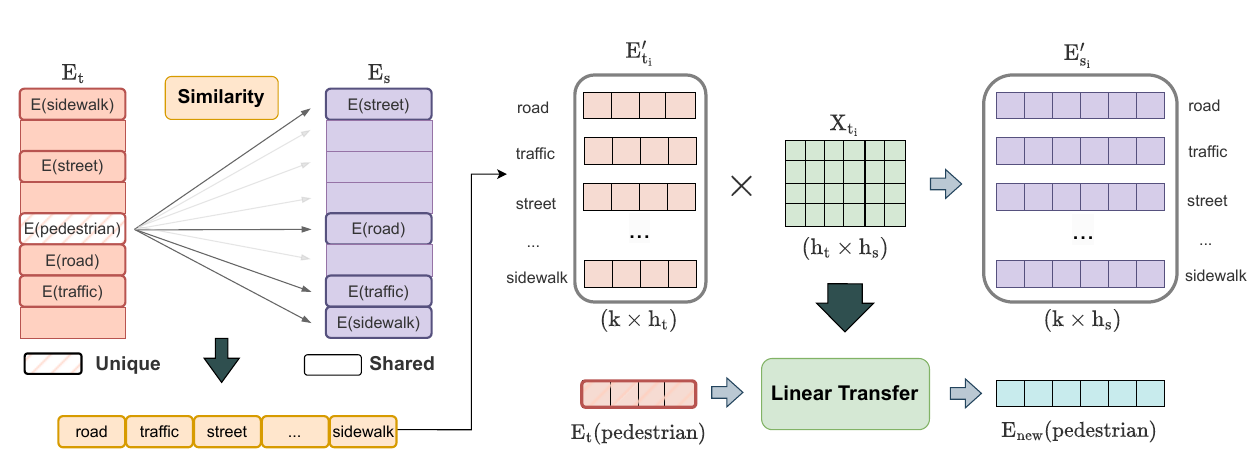
\includegraphics[width=\textwidth]{images/salt-summary.png}
  \caption[Sơ đồ tổng quan SALT]{Sơ đồ tổng quan SALT: token không trùng được ánh xạ thông
    qua các token neo gần về ngữ nghĩa trong phần từ vựng chồng lấp, sau đó dùng hồi quy
    tuyến tính cục bộ để chuyển nhúng sang không gian mô hình nguồn. Hình trích từ Lee và
    cộng sự~\cite{lee2025salt}.}
  \label{fig:salt-summary}
\end{figure}

Trong nghiên cứu gốc, SALT chủ yếu được kiểm chứng trên các mô hình dạng decoder như Gemma
và XGLM. Đề tài kế thừa ý tưởng này nhưng áp dụng vào bối cảnh khác: mô hình nền là NeoBERT
Encoder-only, ngôn ngữ đích là tiếng Việt, và lớp đầu ra của NeoBERT cần được xử lý như một
ma trận riêng. Các điều chỉnh cụ thể được trình bày trong Chương~\ref{chap:method}.

% ======================================================================
\section{Nhận xét định hướng}
\label{sec:related-summary}

Từ các cơ sở trên, chúng tôi xem NeoBERT là một nền tảng phù hợp để xây dựng Encoder tiếng
Việt hiện đại: phần thân Transformer đã mạnh, hỗ trợ ngữ cảnh dài, nhưng lớp từ vựng và
không gian đầu vào vẫn mang thiên lệch tiếng Anh. Vì vậy, hướng tiếp cận hợp lý không phải
huấn luyện lại từ đầu, mà là tái sử dụng phần thân NeoBERT và khởi tạo lại lớp nhúng tiếng
Việt một cách có thông tin.

Nhận xét quan trọng nhất của chúng tôi là bước khởi tạo không gian nhúng quyết định chất
lượng thích nghi ban đầu. Nếu điểm khởi đầu lệch quá xa không gian NeoBERT, quá trình CPT
dễ tiêu tốn tài nguyên để sửa lỗi căn chỉnh thay vì học tiếng Việt. Do đó, Chương~\ref{chap:method}
sẽ tập trung vào một biến thể SALT phù hợp với NeoBERT, bao gồm lựa chọn tập neo, chiếu cục
bộ, xử lý lớp đầu ra tách rời và hiệu chỉnh chuẩn của nhúng.
